% =====================================================================
% figA2  — R/ggplot2 -> tikzDevice (parallel to ../figures-tex/figA2_crossarch.tex)
% Canonical-JSON-only. Regenerate: Rscript figures/make_figures_ieee.R
% Provenance (JSON path :: field = plotted value), one line per series:
% SOURCE: results/G1_L12_analysis.json :: aggregate.within_probe_mean_across_seeds = 0.6018
% SOURCE: results/C3_null_llama3b_L14.json :: aggregate.within_probe_mean_across_seeds = 0.2910
% SOURCE: results/C3_null_gemma2b_L13_v2.json :: aggregate.within_probe_mean_across_seeds = 0.0841
% SOURCE: results/C3_null_phi35_L16_v2.json :: aggregate.within_probe_mean_across_seeds = 0.0169
% SOURCE: results/C3_null_qwen05b_L12.json :: aggregate.within_probe_mean_across_seeds = 0.1030
% SOURCE: results/C3_null_qwen15b_L14.json :: aggregate.within_probe_mean_across_seeds = -0.1716
% SOURCE: results/C3_null_qwen3b_L18_v2.json :: aggregate.within_probe_mean_across_seeds = -0.1191
% SOURCE: results/C1_magnitude_table.json :: families[family=llama1b_L12].within_probe_mean_abs_across_seeds = 0.6133
% SOURCE: results/C1_magnitude_table.json :: families[family=gemma2b_L13].within_probe_mean_abs_across_seeds = 0.0858
% SOURCE: results/C1_magnitude_table.json :: families[family=phi35_L16].within_probe_mean_abs_across_seeds = 0.3214
% SOURCE: results/C1_magnitude_table.json :: families[family=qwen05b_L12].within_probe_mean_abs_across_seeds = 0.3197
% SOURCE: results/C1_magnitude_table.json :: families[family=qwen15b_L14].within_probe_mean_abs_across_seeds = 0.4124
% SOURCE: results/C1_magnitude_table.json :: families[family=qwen3b_L18].within_probe_mean_abs_across_seeds = 0.4013
% =====================================================================
% !TEX encoding = UTF-8 Unicode
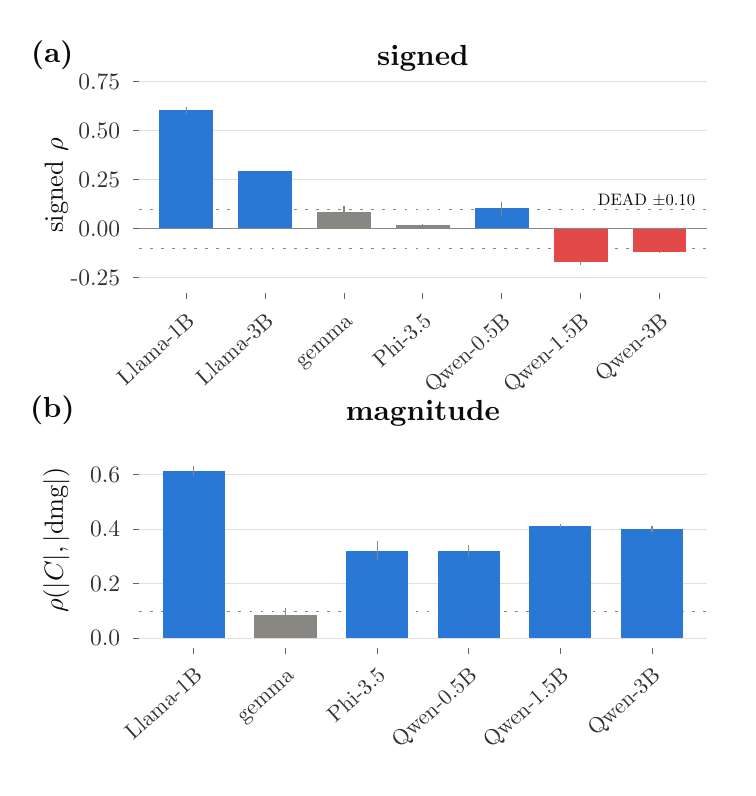
\begin{tikzpicture}[x=1pt,y=1pt]
\definecolor{fillColor}{RGB}{255,255,255}
\path[use as bounding box,fill=fillColor,fill opacity=0.00] (0,0) rectangle (252.94,267.40);
\begin{scope}
\path[clip] (  0.00,  0.00) rectangle (252.94,267.40);
\definecolor{drawColor}{RGB}{255,255,255}
\definecolor{fillColor}{RGB}{255,255,255}

\path[draw=drawColor,line width= 0.6pt,line join=round,line cap=round,fill=fillColor] (  0.00,  0.00) rectangle (252.94,267.40);
\end{scope}
\begin{scope}
\path[clip] (  5.50,133.70) rectangle (247.44,261.90);
\definecolor{fillColor}{RGB}{255,255,255}

\path[fill=fillColor] (  5.50,133.70) rectangle (247.44,261.90);
\end{scope}
\begin{scope}
\path[clip] (  5.50,  5.50) rectangle (247.44,133.70);
\definecolor{fillColor}{RGB}{255,255,255}

\path[fill=fillColor] (  5.50,  5.50) rectangle (247.44,133.70);
\end{scope}
\begin{scope}
\path[clip] ( 40.17,171.41) rectangle (245.44,249.39);
\definecolor{drawColor}{RGB}{225,224,217}

\path[draw=drawColor,line width= 0.3pt,line join=round] ( 40.17,177.08) --
	(245.44,177.08);

\path[draw=drawColor,line width= 0.3pt,line join=round] ( 40.17,194.80) --
	(245.44,194.80);

\path[draw=drawColor,line width= 0.3pt,line join=round] ( 40.17,212.53) --
	(245.44,212.53);

\path[draw=drawColor,line width= 0.3pt,line join=round] ( 40.17,230.25) --
	(245.44,230.25);

\path[draw=drawColor,line width= 0.3pt,line join=round] ( 40.17,247.97) --
	(245.44,247.97);
\definecolor{drawColor}{RGB}{137,135,129}

\path[draw=drawColor,line width= 0.3pt,dash pattern=on 1pt off 3pt ,line join=round] ( 40.17,187.71) -- (245.44,187.71);

\path[draw=drawColor,line width= 0.3pt,dash pattern=on 1pt off 3pt ,line join=round] ( 40.17,201.89) -- (245.44,201.89);
\definecolor{fillColor}{RGB}{42,120,214}

\path[fill=fillColor] ( 47.58,194.80) rectangle ( 66.97,237.47);

\path[fill=fillColor] ( 76.09,194.80) rectangle ( 95.48,215.43);
\definecolor{fillColor}{RGB}{137,135,129}

\path[fill=fillColor] (104.60,194.80) rectangle (123.99,200.77);

\path[fill=fillColor] (133.11,194.80) rectangle (152.50,196.00);
\definecolor{fillColor}{RGB}{42,120,214}

\path[fill=fillColor] (161.63,194.80) rectangle (181.01,202.11);
\definecolor{fillColor}{RGB}{227,73,72}

\path[fill=fillColor] (190.14,182.64) rectangle (209.52,194.80);

\path[fill=fillColor] (218.65,186.36) rectangle (238.03,194.80);

\path[draw=drawColor,line width= 0.3pt,line join=round] ( 40.17,194.80) -- (245.44,194.80);

\path[draw=drawColor,line width= 0.4pt,line join=round] ( 57.28,238.81) --
	( 57.28,238.81);

\path[draw=drawColor,line width= 0.4pt,line join=round] ( 57.28,238.81) --
	( 57.28,236.13);

\path[draw=drawColor,line width= 0.4pt,line join=round] ( 57.28,236.13) --
	( 57.28,236.13);

\path[draw=drawColor,line width= 0.4pt,line join=round] (114.30,202.85) --
	(114.30,202.85);

\path[draw=drawColor,line width= 0.4pt,line join=round] (114.30,202.85) --
	(114.30,198.68);

\path[draw=drawColor,line width= 0.4pt,line join=round] (114.30,198.68) --
	(114.30,198.68);

\path[draw=drawColor,line width= 0.4pt,line join=round] (142.81,196.63) --
	(142.81,196.63);

\path[draw=drawColor,line width= 0.4pt,line join=round] (142.81,196.63) --
	(142.81,195.38);

\path[draw=drawColor,line width= 0.4pt,line join=round] (142.81,195.38) --
	(142.81,195.38);

\path[draw=drawColor,line width= 0.4pt,line join=round] (171.32,204.44) --
	(171.32,204.44);

\path[draw=drawColor,line width= 0.4pt,line join=round] (171.32,204.44) --
	(171.32,199.77);

\path[draw=drawColor,line width= 0.4pt,line join=round] (171.32,199.77) --
	(171.32,199.77);

\path[draw=drawColor,line width= 0.4pt,line join=round] (199.83,183.52) --
	(199.83,183.52);

\path[draw=drawColor,line width= 0.4pt,line join=round] (199.83,183.52) --
	(199.83,181.75);

\path[draw=drawColor,line width= 0.4pt,line join=round] (199.83,181.75) --
	(199.83,181.75);

\path[draw=drawColor,line width= 0.4pt,line join=round] (228.34,186.84) --
	(228.34,186.84);

\path[draw=drawColor,line width= 0.4pt,line join=round] (228.34,186.84) --
	(228.34,185.88);

\path[draw=drawColor,line width= 0.4pt,line join=round] (228.34,185.88) --
	(228.34,185.88);
\definecolor{drawColor}{RGB}{11,11,11}

\node[text=drawColor,anchor=base east,inner sep=0pt, outer sep=0pt, scale=  0.60] at (241.17,203.14) {DEAD $\pm$0.10};
\end{scope}
\begin{scope}
\path[clip] (  0.00,  0.00) rectangle (252.94,267.40);
\definecolor{drawColor}{gray}{0.20}

\node[text=drawColor,anchor=base east,inner sep=0pt, outer sep=0pt, scale=  0.85] at ( 33.45,174.31) {-0.25};

\node[text=drawColor,anchor=base east,inner sep=0pt, outer sep=0pt, scale=  0.85] at ( 33.45,192.04) {0.00};

\node[text=drawColor,anchor=base east,inner sep=0pt, outer sep=0pt, scale=  0.85] at ( 33.45,209.76) {0.25};

\node[text=drawColor,anchor=base east,inner sep=0pt, outer sep=0pt, scale=  0.85] at ( 33.45,227.48) {0.50};

\node[text=drawColor,anchor=base east,inner sep=0pt, outer sep=0pt, scale=  0.85] at ( 33.45,245.21) {0.75};
\end{scope}
\begin{scope}
\path[clip] (  0.00,  0.00) rectangle (252.94,267.40);
\definecolor{drawColor}{gray}{0.40}

\path[draw=drawColor,line width= 0.3pt,line join=round] ( 38.17,177.08) --
	( 40.17,177.08);

\path[draw=drawColor,line width= 0.3pt,line join=round] ( 38.17,194.80) --
	( 40.17,194.80);

\path[draw=drawColor,line width= 0.3pt,line join=round] ( 38.17,212.53) --
	( 40.17,212.53);

\path[draw=drawColor,line width= 0.3pt,line join=round] ( 38.17,230.25) --
	( 40.17,230.25);

\path[draw=drawColor,line width= 0.3pt,line join=round] ( 38.17,247.97) --
	( 40.17,247.97);
\end{scope}
\begin{scope}
\path[clip] (  0.00,  0.00) rectangle (252.94,267.40);
\definecolor{drawColor}{gray}{0.40}

\path[draw=drawColor,line width= 0.3pt,line join=round] ( 57.28,169.41) --
	( 57.28,171.41);

\path[draw=drawColor,line width= 0.3pt,line join=round] ( 85.79,169.41) --
	( 85.79,171.41);

\path[draw=drawColor,line width= 0.3pt,line join=round] (114.30,169.41) --
	(114.30,171.41);

\path[draw=drawColor,line width= 0.3pt,line join=round] (142.81,169.41) --
	(142.81,171.41);

\path[draw=drawColor,line width= 0.3pt,line join=round] (171.32,169.41) --
	(171.32,171.41);

\path[draw=drawColor,line width= 0.3pt,line join=round] (199.83,169.41) --
	(199.83,171.41);

\path[draw=drawColor,line width= 0.3pt,line join=round] (228.34,169.41) --
	(228.34,171.41);
\end{scope}
\begin{scope}
\path[clip] (  0.00,  0.00) rectangle (252.94,267.40);
\definecolor{drawColor}{gray}{0.20}

\node[text=drawColor,rotate= 42.00,anchor=base east,inner sep=0pt, outer sep=0pt, scale=  0.80] at ( 60.76,160.81) {Llama-1B};

\node[text=drawColor,rotate= 42.00,anchor=base east,inner sep=0pt, outer sep=0pt, scale=  0.80] at ( 89.27,160.81) {Llama-3B};

\node[text=drawColor,rotate= 42.00,anchor=base east,inner sep=0pt, outer sep=0pt, scale=  0.80] at (117.78,160.81) {gemma};

\node[text=drawColor,rotate= 42.00,anchor=base east,inner sep=0pt, outer sep=0pt, scale=  0.80] at (146.29,160.81) {Phi-3.5};

\node[text=drawColor,rotate= 42.00,anchor=base east,inner sep=0pt, outer sep=0pt, scale=  0.80] at (174.80,160.81) {Qwen-0.5B};

\node[text=drawColor,rotate= 42.00,anchor=base east,inner sep=0pt, outer sep=0pt, scale=  0.80] at (203.31,160.81) {Qwen-1.5B};

\node[text=drawColor,rotate= 42.00,anchor=base east,inner sep=0pt, outer sep=0pt, scale=  0.80] at (231.82,160.81) {Qwen-3B};
\end{scope}
\begin{scope}
\path[clip] (  0.00,  0.00) rectangle (252.94,267.40);
\definecolor{drawColor}{RGB}{11,11,11}

\node[text=drawColor,rotate= 90.00,anchor=base,inner sep=0pt, outer sep=0pt, scale=  0.95] at ( 12.68,210.40) {signed $\rho$};
\end{scope}
\begin{scope}
\path[clip] (  0.00,  0.00) rectangle (252.94,267.40);
\definecolor{drawColor}{RGB}{11,11,11}

\node[text=drawColor,anchor=base,inner sep=0pt, outer sep=0pt, scale=  1.05] at (142.81,253.66) {\bfseries signed};
\end{scope}
\begin{scope}
\path[clip] (  0.00,  0.00) rectangle (252.94,267.40);
\definecolor{drawColor}{RGB}{11,11,11}

\node[text=drawColor,anchor=base,inner sep=0pt, outer sep=0pt, scale=  1.05] at (  8.89,254.76) {\bfseries (a)};
\end{scope}
\begin{scope}
\path[clip] ( 40.17, 43.21) rectangle (245.44,121.19);
\definecolor{drawColor}{RGB}{225,224,217}

\path[draw=drawColor,line width= 0.3pt,line join=round] ( 40.17, 46.75) --
	(245.44, 46.75);

\path[draw=drawColor,line width= 0.3pt,line join=round] ( 40.17, 66.45) --
	(245.44, 66.45);

\path[draw=drawColor,line width= 0.3pt,line join=round] ( 40.17, 86.14) --
	(245.44, 86.14);

\path[draw=drawColor,line width= 0.3pt,line join=round] ( 40.17,105.83) --
	(245.44,105.83);
\definecolor{drawColor}{RGB}{137,135,129}

\path[draw=drawColor,line width= 0.3pt,dash pattern=on 1pt off 3pt ,line join=round] ( 40.17, 56.60) -- (245.44, 56.60);
\definecolor{fillColor}{RGB}{42,120,214}

\path[fill=fillColor] ( 48.78, 46.75) rectangle ( 71.29,107.14);
\definecolor{fillColor}{RGB}{137,135,129}

\path[fill=fillColor] ( 81.89, 46.75) rectangle (104.40, 55.20);
\definecolor{fillColor}{RGB}{42,120,214}

\path[fill=fillColor] (115.00, 46.75) rectangle (137.51, 78.40);

\path[fill=fillColor] (148.11, 46.75) rectangle (170.62, 78.23);

\path[fill=fillColor] (181.21, 46.75) rectangle (203.73, 87.36);

\path[fill=fillColor] (214.32, 46.75) rectangle (236.84, 86.27);

\path[draw=drawColor,line width= 0.4pt,line join=round] ( 60.04,108.97) --
	( 60.04,108.97);

\path[draw=drawColor,line width= 0.4pt,line join=round] ( 60.04,108.97) --
	( 60.04,105.31);

\path[draw=drawColor,line width= 0.4pt,line join=round] ( 60.04,105.31) --
	( 60.04,105.31);

\path[draw=drawColor,line width= 0.4pt,line join=round] ( 93.15, 57.66) --
	( 93.15, 57.66);

\path[draw=drawColor,line width= 0.4pt,line join=round] ( 93.15, 57.66) --
	( 93.15, 52.74);

\path[draw=drawColor,line width= 0.4pt,line join=round] ( 93.15, 52.74) --
	( 93.15, 52.74);

\path[draw=drawColor,line width= 0.4pt,line join=round] (126.25, 81.86) --
	(126.25, 81.86);

\path[draw=drawColor,line width= 0.4pt,line join=round] (126.25, 81.86) --
	(126.25, 74.94);

\path[draw=drawColor,line width= 0.4pt,line join=round] (126.25, 74.94) --
	(126.25, 74.94);

\path[draw=drawColor,line width= 0.4pt,line join=round] (159.36, 80.32) --
	(159.36, 80.32);

\path[draw=drawColor,line width= 0.4pt,line join=round] (159.36, 80.32) --
	(159.36, 76.15);

\path[draw=drawColor,line width= 0.4pt,line join=round] (159.36, 76.15) --
	(159.36, 76.15);

\path[draw=drawColor,line width= 0.4pt,line join=round] (192.47, 88.21) --
	(192.47, 88.21);

\path[draw=drawColor,line width= 0.4pt,line join=round] (192.47, 88.21) --
	(192.47, 86.51);

\path[draw=drawColor,line width= 0.4pt,line join=round] (192.47, 86.51) --
	(192.47, 86.51);

\path[draw=drawColor,line width= 0.4pt,line join=round] (225.58, 87.35) --
	(225.58, 87.35);

\path[draw=drawColor,line width= 0.4pt,line join=round] (225.58, 87.35) --
	(225.58, 85.18);

\path[draw=drawColor,line width= 0.4pt,line join=round] (225.58, 85.18) --
	(225.58, 85.18);
\end{scope}
\begin{scope}
\path[clip] (  0.00,  0.00) rectangle (252.94,267.40);
\definecolor{drawColor}{gray}{0.20}

\node[text=drawColor,anchor=base east,inner sep=0pt, outer sep=0pt, scale=  0.85] at ( 33.45, 43.99) {0.0};

\node[text=drawColor,anchor=base east,inner sep=0pt, outer sep=0pt, scale=  0.85] at ( 33.45, 63.68) {0.2};

\node[text=drawColor,anchor=base east,inner sep=0pt, outer sep=0pt, scale=  0.85] at ( 33.45, 83.37) {0.4};

\node[text=drawColor,anchor=base east,inner sep=0pt, outer sep=0pt, scale=  0.85] at ( 33.45,103.07) {0.6};
\end{scope}
\begin{scope}
\path[clip] (  0.00,  0.00) rectangle (252.94,267.40);
\definecolor{drawColor}{gray}{0.40}

\path[draw=drawColor,line width= 0.3pt,line join=round] ( 38.17, 46.75) --
	( 40.17, 46.75);

\path[draw=drawColor,line width= 0.3pt,line join=round] ( 38.17, 66.45) --
	( 40.17, 66.45);

\path[draw=drawColor,line width= 0.3pt,line join=round] ( 38.17, 86.14) --
	( 40.17, 86.14);

\path[draw=drawColor,line width= 0.3pt,line join=round] ( 38.17,105.83) --
	( 40.17,105.83);
\end{scope}
\begin{scope}
\path[clip] (  0.00,  0.00) rectangle (252.94,267.40);
\definecolor{drawColor}{gray}{0.40}

\path[draw=drawColor,line width= 0.3pt,line join=round] ( 60.04, 41.21) --
	( 60.04, 43.21);

\path[draw=drawColor,line width= 0.3pt,line join=round] ( 93.15, 41.21) --
	( 93.15, 43.21);

\path[draw=drawColor,line width= 0.3pt,line join=round] (126.25, 41.21) --
	(126.25, 43.21);

\path[draw=drawColor,line width= 0.3pt,line join=round] (159.36, 41.21) --
	(159.36, 43.21);

\path[draw=drawColor,line width= 0.3pt,line join=round] (192.47, 41.21) --
	(192.47, 43.21);

\path[draw=drawColor,line width= 0.3pt,line join=round] (225.58, 41.21) --
	(225.58, 43.21);
\end{scope}
\begin{scope}
\path[clip] (  0.00,  0.00) rectangle (252.94,267.40);
\definecolor{drawColor}{gray}{0.20}

\node[text=drawColor,rotate= 42.00,anchor=base east,inner sep=0pt, outer sep=0pt, scale=  0.80] at ( 63.52, 32.61) {Llama-1B};

\node[text=drawColor,rotate= 42.00,anchor=base east,inner sep=0pt, outer sep=0pt, scale=  0.80] at ( 96.63, 32.61) {gemma};

\node[text=drawColor,rotate= 42.00,anchor=base east,inner sep=0pt, outer sep=0pt, scale=  0.80] at (129.74, 32.61) {Phi-3.5};

\node[text=drawColor,rotate= 42.00,anchor=base east,inner sep=0pt, outer sep=0pt, scale=  0.80] at (162.85, 32.61) {Qwen-0.5B};

\node[text=drawColor,rotate= 42.00,anchor=base east,inner sep=0pt, outer sep=0pt, scale=  0.80] at (195.96, 32.61) {Qwen-1.5B};

\node[text=drawColor,rotate= 42.00,anchor=base east,inner sep=0pt, outer sep=0pt, scale=  0.80] at (229.06, 32.61) {Qwen-3B};
\end{scope}
\begin{scope}
\path[clip] (  0.00,  0.00) rectangle (252.94,267.40);
\definecolor{drawColor}{RGB}{11,11,11}

\node[text=drawColor,rotate= 90.00,anchor=base,inner sep=0pt, outer sep=0pt, scale=  0.95] at ( 12.68, 82.20) {$\rho(|C|,|$dmg$|)$};
\end{scope}
\begin{scope}
\path[clip] (  0.00,  0.00) rectangle (252.94,267.40);
\definecolor{drawColor}{RGB}{11,11,11}

\node[text=drawColor,anchor=base,inner sep=0pt, outer sep=0pt, scale=  1.05] at (142.81,125.47) {\bfseries magnitude};
\end{scope}
\begin{scope}
\path[clip] (  0.00,  0.00) rectangle (252.94,267.40);
\definecolor{drawColor}{RGB}{11,11,11}

\node[text=drawColor,anchor=base,inner sep=0pt, outer sep=0pt, scale=  1.05] at (  8.89,126.56) {\bfseries (b)};
\end{scope}
\end{tikzpicture}
